% Created 2024-11-04 Mon 19:14
% Intended LaTeX compiler: lualatex
\documentclass[xcolor=table,10pt,aspectratio=169]{beamer}

\RequirePackage[l2tabu,orthodox]{nag}            %% Warn about obsolete commands and packages
\RequirePackage{amsmath,amsfonts,amssymb,amsthm} %% Math
\RequirePackage{ifpdf,ifxetex,ifluatex}          %% Detect XeTeX and LuaTeX
\RequirePackage{xspace}
\RequirePackage{graphicx}
\RequirePackage{comment}
\RequirePackage{url}
\RequirePackage{relsize}
\RequirePackage{booktabs}
\RequirePackage{tabularx}
\RequirePackage[normalem]{ulem}
\ifluatex%
\else%
  \RequirePackage[all]{xy}
\fi%
\RequirePackage{etoolbox}
\RequirePackage{csquotes}
\RequirePackage[export]{adjustbox}

\RequirePackage{silence}
\WarningsOff[microtype]
\WarningFilter{microtype}{Unknown slot}

% https://tex.stackexchange.com/questions/64459/overfull-vbox-warning-disable
\vfuzz=30pt
\hfuzz=30pt


%%%
%%% Code Listings
%%%

\RequirePackage{listings}
\lstdefinelanguage{Sage}[]{Python}{morekeywords={True,False,sage,cdef,cpdef,ctypedef,self},sensitive=true}

\lstset{frame=none,
  showtabs=False,
  showspaces=False,
  showstringspaces=False,
  commentstyle={\color{gray}},
  keywordstyle={\color{mLightBrown}\textbf},
  stringstyle ={\color{mDarkBrown}},
  frame=single,
  basicstyle=\tt\scriptsize\relax,
  backgroundcolor=\color{gray!190!black},
  inputencoding=utf8,
  literate={…}{{\ldots}}1,
  belowskip=0.0em,
}

\makeatletter
\patchcmd{\@verbatim}
  {\verbatim@font}
  {\verbatim@font\scriptsize}
  {}{}
\makeatother


%%%
%%% Pseudocode
%%%

\let\nl\undefine
\let\procedure\relax
\let\endprocedure\relax
\usepackage{algorithm2e}

%%%
%%% Tikz
%%%

\RequirePackage{tikz,pgfplots}
\pgfplotsset{compat=newest}

\usetikzlibrary{calc}
\usetikzlibrary{arrows}
\usetikzlibrary{automata}
\usetikzlibrary{positioning}
\usetikzlibrary{decorations.pathmorphing}
\usetikzlibrary{backgrounds}
\usetikzlibrary{fit,}
\usetikzlibrary{shapes.symbols}
\usetikzlibrary{chains}
\usetikzlibrary{shapes.geometric}
\usetikzlibrary{shapes.arrows}
\usetikzlibrary{graphs}

%% Cache but disable by default

\usetikzlibrary{external}
\tikzset{external/export=false}

\definecolor{DarkPurple}{HTML}{332288}
\definecolor{DarkBlue}{HTML}{6699CC}
\definecolor{LightBlue}{HTML}{88CCEE}
\definecolor{DarkGreen}{HTML}{117733}
\definecolor{DarkRed}{HTML}{661100}
\definecolor{LightRed}{HTML}{CC6677}
\definecolor{LightPink}{HTML}{AA4466}
\definecolor{DarkPink}{HTML}{882255}
\definecolor{LightPurple}{HTML}{AA4499}
\definecolor{DarkBrown}{HTML}{604c38}
\definecolor{DarkTeal}{HTML}{23373b}
\definecolor{LightBrown}{HTML}{EB811B}
\definecolor{LightGreen}{HTML}{14B03D}
\definecolor{DarkOrange}{HTML}{FFDD00}

\pgfplotsset{width=1.0\textwidth,
  height=0.6\textwidth,
  cycle list={%
    solid,LightGreen,thick\\%
    dotted,LightRed,very thick\\%
    dashed,DarkBlue,thick\\%
    dashdotted,DarkPink,thick\\%
    dashdotdotted,LightGreen,thick\\%
    loosely dotted,very thick\\%
    loosely dashed,DarkBlue,very thick\\%
    loosely dashdotted,DarkPink,very thick\\%
    \\%
    DarkBrown,thick\\%
  },
  legend pos=north west,
  legend cell align={left}}

\pgfplotsset{select coords between index/.style 2 args={
    x filter/.code={
        \ifnum\coordindex<#1\def\pgfmathresult{}\fi
        \ifnum\coordindex>#2\def\pgfmathresult{}\fi
    }
}}

\setlength{\marginparwidth}{2cm}
\pgfplotsset{compat=1.18}

%%%
%%% SVG (Inkscape)
%%%

\ifpdf% 
\providecommand{\executeiffilenewer}[3]{%
  \ifnum\pdfstrcmp{\pdffilemoddate{#1}}%
    {\pdffilemoddate{#2}}>0%
    {\immediate\write18{#3}}
  \fi%
}
\else%
\providecommand{\executeiffilenewer}[3]{%
  {\immediate\write18{#3}} % hack
}
\fi%

\providecommand{\includesvg}[2][1.0\textwidth]{%
 \executeiffilenewer{#1.svg}{#1.pdf}%
 {inkscape -z -D --file=#2.svg --export-pdf=#2.pdf --export-latex --export-area-page}%
 \def\svgwidth{#1} 
 \input{#2.pdf_tex}%
} 

%%%
%%% Attachments
%%%

\RequirePackage{embedfile}


%%%
%%% Metropolis Theme
%%%

\usetheme{metropolis}
\metroset{color/block=fill}
\metroset{numbering=none}
\metroset{outer/progressbar=foot}
\metroset{titleformat=smallcaps}

\setbeamercolor{description item}{fg=mLightBrown}
\setbeamerfont{footnote}{size=\scriptsize}
\setbeamercolor{example text}{fg=mDarkBrown}
\setbeamercolor{block title alerted}{fg=white, bg=mDarkBrown}
\setbeamerfont{alerted text}{series=\ifmmode\boldmath\else\bfseries\fi}

\renewcommand*{\UrlFont}{\ttfamily\relax}

%%%
%%% UTF-8 & Fonts
%%% 

\RequirePackage{unicodesymbols} % after metropolis which loads fontspec

\ifboolexpr{bool{xetex} or bool{luatex}}{%
\setmonofont[BoldFont={Cousine Bold},
             ItalicFont={Cousine Italic},
             BoldItalicFont={Cousine Bold Italic},
             Scale=0.9]{Cousine}             
}{%
}

%%%
%%% BibLaTeX
%%%

\RequirePackage[backend=bibtex,
            style=alphabetic,
            maxnames=8,maxbibnames=8,maxalphanames=8,
            citestyle=alphabetic]{biblatex}

\bibliography{local.bib,abbrev3.bib,crypto_crossref.bib,rfc.bib,jacm.bib,dcc.bib}

\setbeamertemplate{bibliography item}[text]
% https://tex.stackexchange.com/questions/683533/beamer-theme-metropolis-does-not-allow-different-font-size-for-fullcite
\setbeamerfont{bibliography entry title}{size=}
\setbeamerfont{bibliography entry author}{size=}
\setbeamerfont{bibliography entry location}{size=}
\setbeamerfont{bibliography entry note}{size=}

\DeclareFieldFormat{title}{\alert{#1}}
\DeclareFieldFormat[book]{title}{\alert{#1}}
\DeclareFieldFormat[thesis]{title}{\alert{#1}}
\DeclareFieldFormat[inproceedings]{title}{\alert{#1}}
\DeclareFieldFormat[incollection]{title}{\alert{#1}}
\DeclareFieldFormat[article]{title}{\alert{#1}}
\DeclareFieldFormat[misc]{title}{\alert{#1}}

%%% 
%%% Microtype
%%%

\IfFileExists{upquote.sty}{\RequirePackage{upquote}}{}
\IfFileExists{microtype.sty}{\RequirePackage{microtype}}{}
\IfFileExists{microtype.sty}{\PassOptionsToPackage{verbose=silent}{microtype}}{}

\setlength{\parindent}{0pt}                   %%
\setlength{\parskip}{6pt plus 2pt minus 1pt}  %%
\setlength{\emergencystretch}{3em}            %% prevent overfull lines
\setcounter{secnumdepth}{0}                   %%

%%%
%%% Maths
%%%

\DeclareMathOperator{\Vol}{Vol}
\DeclareMathOperator{\vol}{vol}
\DeclareMathOperator{\GH}{GH}
\renewcommand{\vec}[1]{\ensuremath{\mathbf{#1}}\xspace}
\newcommand{\norm}[1]{\left\lVert#1\right\rVert}
\providecommand{\mat}[1]{\ensuremath{\vec{#1}}\xspace}
\providecommand{\ring}[0]{\ensuremath{\mathcal{R}}\xspace}


\usepackage{graphicx}
\usepackage{longtable}
\usepackage{wrapfig}
\usepackage{rotating}
\usepackage[normalem]{ulem}
\usepackage{amsmath}
\usepackage{amssymb}
\usepackage{capt-of}
\usepackage{hyperref}
\usepackage{booktabs}
\usepackage{microtype}
\usepackage{newunicodechar}
\usepackage[notions,operators,sets,keys,ff,adversary,primitives,complexity,asymptotics,lambda,landau,advantage]{cryptocode}
\usepackage[capitalize]{cleveref}
\usepackage[,]{stmaryrd}
\usepackage[british]{babel}
\usepackage{xspace}
\usepackage{units}
\usepackage{nicefrac}
\usepackage{gensymb}
\usepackage{amsthm}
\usepackage{amsmath}
\usepackage{amssymb}
\usepackage{xcolor}
\usepackage{listings}
\usepackage[color=cyan!0!magenta!4!yellow!16]{todonotes}
% \tikzset{external/export=true}
\newcommand{\randkHSIS}{\ensuremath{\$\pcmathhyphen{}\mathsf{kHSIS}}\xspace}
\newcommand{\kHISIS}{\ensuremath{\mathsf{kHISIS}}\xspace}
\newcommand{\MSIS}{\ensuremath{\mathsf{M}\pcmathhyphen{}\mathsf{SIS}}\xspace}
\newcommand{\MISIS}{\ensuremath{\mathsf{M}\pcmathhyphen{}\mathsf{ISIS}}\xspace}
\newcommand{\SIVP}{\ensuremath{\mathsf{SIVP}}\xspace}
\newfontfamily{\fallbackfont}{Linux Libertine O}[Scale=MatchLowercase]
\DeclareTextFontCommand{\textfallback}{\fallbackfont}
\newunicodechar{∩}{\textfallback{∩}}
\newcommand{\growthfactor}{\gamma_{\uparrow}}
\newcommand{\shrinkfactor}{\gamma_{\downarrow}}
\newcommand{\combinedfactor}{\gamma}
\usetheme{default}
\author{Martin R. Albrecht}
\date{5 November 2024}
\title{Adventures in SIS with Hints}
\subtitle{Embracing the brave new world where we make it up as we go}
\hypersetup{
pdfauthor={Martin R. Albrecht},
pdftitle={Adventures in SIS with Hints},
pdfkeywords={},
pdfsubject={},
pdfcreator={Emacs 29.4.50 (Org mode 9.6.15)},
pdflang={English},
colorlinks,
citecolor=gray,
filecolor=gray,
linkcolor=gray,
urlcolor=gray
}
\begin{document}

\maketitle

\begin{frame}[label={sec:orgd0ecb85}]{Programme}
\begin{itemize}
\item The \href{https://malb.io/sis-with-hints.html}{SIS with Hints Zoo} is an attempt to keep track of all those new SIS-like assumptions that hand out additional hints.

\item I will discuss several of these assumptions here, with a focus on computational hardness rather than design.

\begin{description}
\item[{Designers}] Please consider whether you can re-use one of those many newfangled assumptions before introducing yet another one.

\item[{Cryptanalysts}] Analyse them!
\end{description}

\item I will also dive a bit deeper into some recent adventures in SIS with hints.
\end{itemize}
\end{frame}

\begin{frame}[label={sec:orge2944ae}]{Teaser}
\begin{center}

\includegraphics[keepaspectratio,height=.9\textheight]{./sis-with-hints-teaser.jpg}
\end{center}
\end{frame}

\begin{frame}[allowframebreaks]{Notation}
\begin{definition}[M-(I)SIS]
\begin{itemize}
\item An instance of \(\MSIS\) is given by \(\mat{A} \sample \ring_q^{n\times m}\) and has solutions \(\vec{u}^{\star} \in \ring^{m}\) such that \(0 < \Vert\vec{u}^{\star} \Vert \leq \beta^{\star}\) and \(\mat{A} \cdot \vec{u}^{\star} \equiv \vec{0} \bmod q\).
\item An instance of \(\MISIS\) is given by \((\mat{A}, \vec{t}) \sample \ring_q^{n\times m} \times \ring_q^n\) and has solutions \(\vec{u}^{\star}\) such that \(0 < \Vert \vec{u}^{\star} \Vert \leq \beta^{\star}\) and \(\mat{A} \cdot \vec{u}^{\star} \equiv \vec{t} \bmod q\).
\end{itemize}
\label{def:sis}
\end{definition}

\begin{itemize}
\item Throughout, feel free to set \(\ring \coloneqq \ZZ\).
\item I am not going to discuss issues arising over cyclotomic rings in any detail.
\end{itemize}

\framebreak

\begin{itemize}
\item The kernel lattice \(\Lambda_q^\bot(\mat{A})\) of \(\mat{A}\) consists of all integral vectors \(\ring_q\)-orthogonal to the rows of \(\mat{A}\):
\[\Lambda_q^\bot(\mat{A}) \coloneqq \set{ \vec{x} \in \ring^m : \mat{A} \cdot \vec{x} \equiv \vec{0} \bmod q }.\]
\item I write \(\mat{G}\) for "the Gadget matrix"
\begin{align*}
\mat{G} &\coloneqq
\left(\begin{array}{*{20}c}
1 & 2 & 4 & \ldots & \lfloor q/2 \rfloor & \ldots & 0 & 0 & 0 & \ldots & 0 \\
\vdots & \vdots & \vdots & \ddots & \vdots       & \ddots & \vdots & \vdots & \vdots & \ddots & \vdots \\
0 & 0 & 0  & \ldots& 0       & \ldots & 1 & 2 & 4 & \ldots & \lfloor q/2 \rfloor \\
\end{array}\right)
\end{align*}
\end{itemize}
\end{frame}

\section{K-SIS}
\label{sec:org3adbde9}

\begin{frame}[label={sec:org962542d}]{The Original: K-SIS}
\begin{definition}
For any integer \(k \geq 0\), an instance of the k-M-SIS problem\footnote{This is the module variant defined in \cite{C:ACLMT22}.} is a matrix \(\mat{A} \sample \ring_{q}^{n \times m}\) and a set of \(k\) vectors \(\vec{u}_{1}, \ldots \vec{u}_{k}\) s.t. \(\mat{A}\cdot \vec{u}_{i} \equiv \vec{0} \bmod q\) with \(\|{\vec{u}_i}\| \leq \beta\). A solution to the problem is a nonzero vector \(\vec{u}^{\star} \in \ring^{m}\) such that
\[\|{\vec{u}^{\star}}\| \leq \beta^*, \quad \mat{A}\cdot \vec{u}^{\star} \equiv \vec{0} \bmod q,\quad \text{and} \quad \vec{u}^{\star} \notin \mathcal{K}\text{-}\operatorname{span}(\set{\vec{u}_i}_{1 \leq i \le k}).\]
\end{definition}

{\footnotesize \fullcite{PKC:BonFre11} \par}
\end{frame}

\begin{frame}[label={sec:orgc7c2e74}]{K-SIS Hardness}
\begin{itemize}
\item \cite{PKC:BonFre11} showed that k-SIS (over \(\ZZ\)) is hard if SIS is hard for discrete Gaussian \(\vec{u}_{i}\) and for \(k = O(1)\).
\item This reduction was improved to cover \(k = \mathcal{O}(m)\).\footfullcite{C:LPSS14}
\item No proof was provided for the module variant in \cite{C:ACLMT22} but Sasha Laphia later proved it for \(k = O(1)\) (unpublished).
\end{itemize}
\end{frame}

\begin{frame}[label={sec:orgf0280cf}]{What can it do?}
\begin{itemize}
\item linearly homomorphic signatures
\item removing the random oracle from GPV signatures at the price of restricting to \(k\) signatures
\item traitor-tracing (by extension to k-LWE\footnote{It is exactly what you think it is})
\item …
\end{itemize}
\end{frame}

\begin{frame}[label={sec:orgf3b51d8}]{Perspective}
\begin{alertblock}{Leakage Resilience}
Alice has \(\mat{A}, \mat{T}\) s.t. \(\mat{T} \in \ring^{m \times m}\) is short and \(\mat{A} \cdot \mat{T} \equiv \mat{0} \bmod q\), i.e. \(\mat{T}\) is trapdoor. Even given, say, \(1/2\) of the columns \(\mat{T}\) it is hard to recover a full trapdoor.
\end{alertblock}
\end{frame}

\section{The Crisis of Knowledge Assumptions}
\label{sec:org4ef4c5e}
\begin{frame}[label={sec:org2a900b8}]{K-R-ISIS}
\begin{definition}[K-M-ISIS Admissible]
Let \(g(\vec{X}) \coloneqq  \vec{X}^{\vec{e}} := \prod_{i \in \ZZ_w} X_i^{e_i}\) for some exponent vector \(\vec{e} \in \ZZ^w\). Let \(\mathcal{G} \subset \mathcal{R}(\vec{X})\) be a set of such monomials with \(k \coloneqq |\mathcal{G}|\). We call a family \(\mathcal{G}\) \textbf{k-M-ISIS-admissible} if all \(g \in \mathcal{G}\) have constant degree, all \(g \in \mathcal{G}\) are distinct and \(0 \not\in\mathcal{G}\).
\end{definition}

\begin{definition}[K-M-ISIS Assumption]
Let \(\vec{t} = (1,0,\ldots,0)\).
Let \(\mathcal{G}\) be k-M-ISIS-admissible.
Let  \(\mat{A} \sample \ring_q^{n \times m}\), \(\vec{v} \sample (\ring_q^\star)^w\). Given \((\mat{A}, \vec{v}, \vec{t}, \{\vec{u}_{g}\})\) with \(\vec{u}_{g}\) short and \(g(\vec{v}) \cdot \vec{t} \equiv \mat{A}\cdot \vec{u}_{g} \bmod q\) it is hard to find a short \(\vec{u}^{\star}\) and small \(s^{\star}\) s.t. \(s^\star \cdot \vec{t} \equiv \mat{A} \cdot \vec{u}^{\star} \bmod q.\)

When \(n = 1\), we call the problem \textbf{K-R-ISIS}.
\end{definition}

{\footnotesize \fullcite{C:ACLMT22} \par}
\end{frame}

\begin{frame}[label={sec:org128496d}]{K-R-ISIS Hardness}
\begin{columns}
\begin{column}[t]{0.65\columnwidth}
\textbf{Some reductions (none cover the interesting cases):}
\begin{itemize}
\item K-R-ISIS is as hard as R-SIS when \(m > k\) or when the system generated by \(\mathcal{G}\) is efficiently invertible.
\item k-M-ISIS is at least as hard as K-R-ISIS: K-M-ISIS is a true generalisation of K-R-SIS.
\item Scaling \((\mathcal{G},g^*)\) multiplicatively by any non-zero \(g\) does not change the hardness: may normalise to \(g^{*} \equiv 1\).
\item \((\mathcal{G},1)\) is as hard as \((\mathcal{G},0)\) for any \(\mathcal{G}\): non-homogeneous variant is no easier than the homogeneous variant.
\end{itemize}
\end{column}

\begin{column}[t]{0.35\columnwidth}
\textbf{Direct cryptanalysis:}
\begin{itemize}
\item a direct SIS attack on \(\mat{A}\).
\item finding short \(\ring\)-linear combinations of \(\vec{u}_{i}\)
\item finding \(\mathcal{K}\)-linear combinations of \(\vec{u}_{i}\) that produce short images.
\end{itemize}

… all seem hard.
\end{column}
\end{columns}
\end{frame}

\begin{frame}[label={sec:orgb77593e}]{Knowledge K-R-ISIS}
The assumption states that for any element \(c \cdot \vec{t}\) that the adversary can produce together with a short preimage, this is some small linear combination of the preimages \(\{\vec{u}_{g}\}\):

\begin{definition}[Knowledge K-R-ISIS]
If an adversary outputs any \(c, \vec{u}_{c}\) s.t.
\[
c \cdot \vec{t} \equiv \mat{A} \cdot \vec{u}_{c} \bmod q
\]

There is an extractor that -- given the adversary's randomness -- outputs short
\(\{c_{g}\}\) s.t.
\[
c \equiv \sum_{g \in \mathcal{G}} c_{g} \cdot g(\vec{v}) \bmod q.
\]
\end{definition}

Think \(\vec{t} = (1,0)\) and the second component serves as a "check equation": The assumption only makes sense for \(n>1\).
\end{frame}

\begin{frame}[label={sec:orgfcdeec2}]{Knowledge K-R-ISIS: The Audacity}
\begin{center}
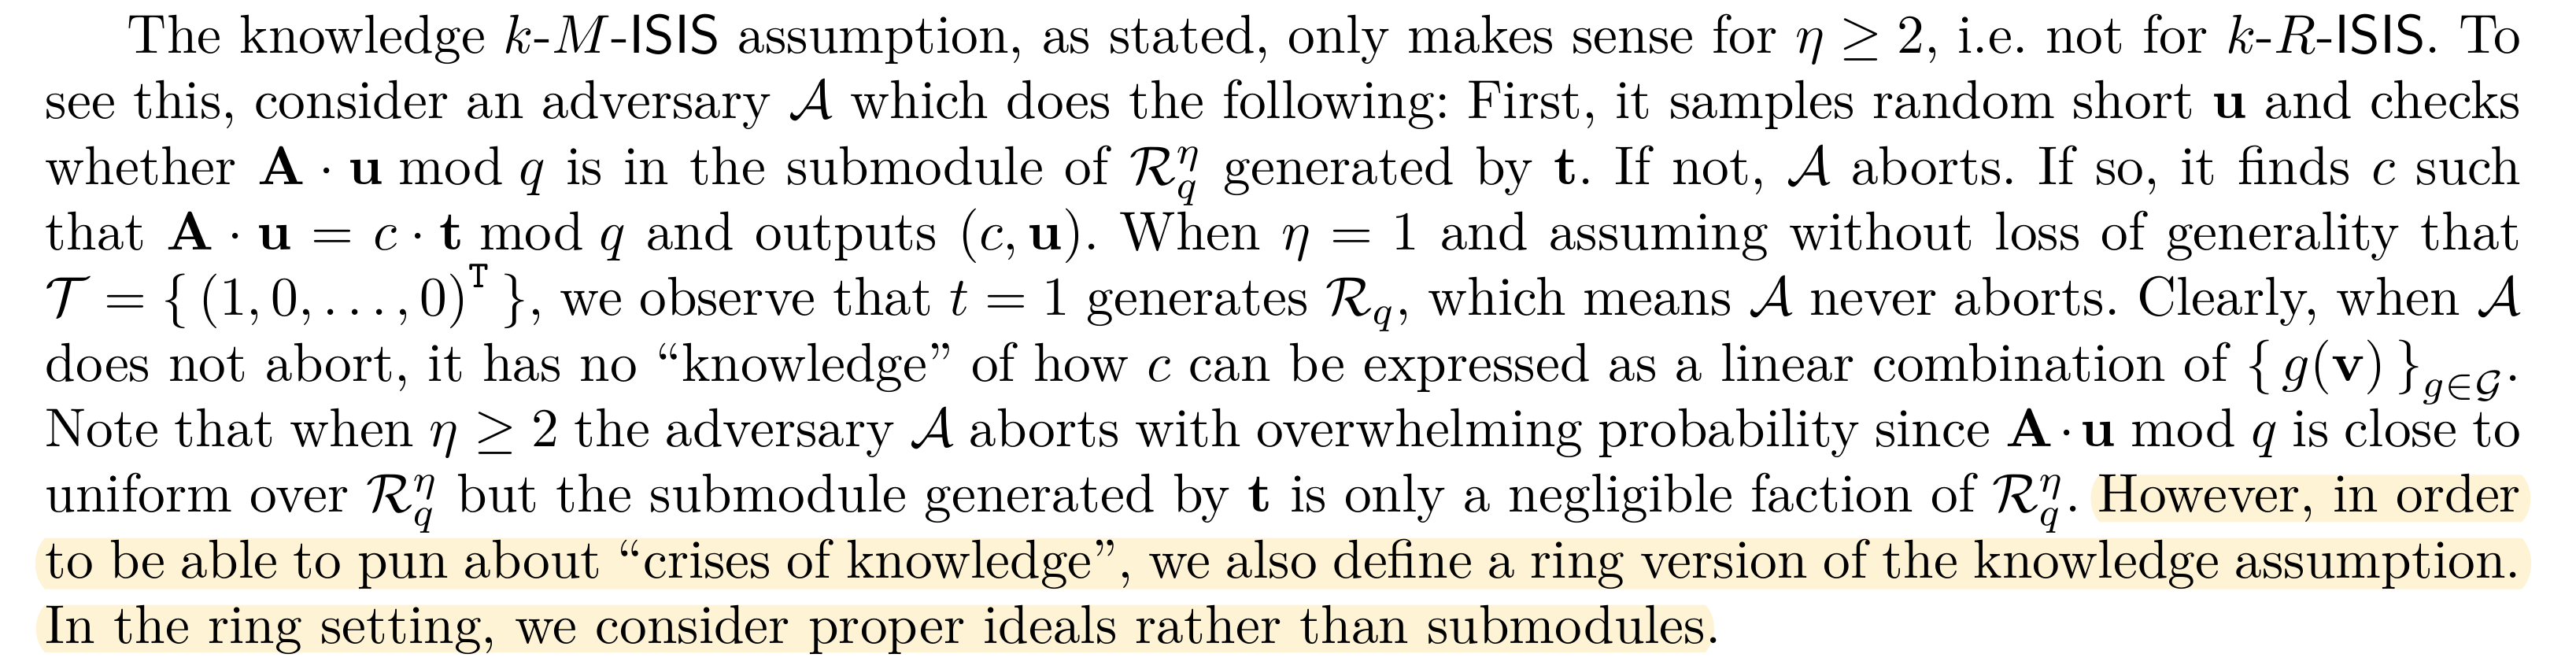
\includegraphics[width=.9\linewidth]{./pun.png}
\end{center}
\end{frame}

\begin{frame}[label={sec:org6a33208}]{Knowledge K-R-ISIS: Almost Instant Karma}
The Knowledge K-M-ISIS assumptions is "morally"\footnote{The assumption is technically unfalsifiable but for all intents and purposes it is wrong by inspection of the attack.} false.

\begin{columns}
\begin{column}{0.3\columnwidth}
\begin{align*}
\begin{pmatrix} \mat{C}\\ \mat{0}\end{pmatrix} \equiv \begin{pmatrix} \mat{A}_{1} \\ \mat{A}_{2} \end{pmatrix} \cdot \mat{U} \bmod q.
\end{align*}
\end{column}

\begin{column}{0.7\columnwidth}
\begin{itemize}
\item \(\mat{U}\) is a trapdoor for \(\mat{A}_{2}\)
\item Use it to find a short preimage of some \((\vec{c}^{\star}, \vec{0})\) using, say, Babai rounding.
\item It will change \(\vec{c}^{\star}\) but we're allowed to output anything in the first component.
\end{itemize}
\end{column}
\end{columns}

{\footnotesize \fullcite{AC:WeeWu23} \par}
\end{frame}

\begin{frame}[label={sec:org84ea0f5}]{Known knowledge assumptions are wrong quantumly}
\begin{quote}
Our main result is a quantum polynomial-time algorithm that samples well-distributed LWE instances while provably not knowing the solution, under the assumption that LWE is hard. Moreover, the approach works for a vast range of LWE parametrizations, including those used in the above-mentioned SNARKs.
\end{quote}

\fullcite{STOC:DebFalSte24}
\end{frame}

\section{BASIS}
\label{sec:orga971918}
\begin{frame}[label={sec:org6efcec1}]{BASIS (Random)}
We consider \(k=2\), for simplicity.

\begin{definition}[BASIS\(_\mathsf{rand}\)]
Let \(\mat{A} \in \ZZ_{q}^{n \times m}\). We're given
\[
\vec{B} := \begin{pmatrix}\mat{A}_{1} & \vec{0} & - \vec{G}\\\vec{0} & \mat{A}_{2} & -\vec{G}\end{pmatrix}
\] and a short \(\vec{T}\) s.t. \(\vec{G} \equiv \vec{B} \cdot \vec{T} \bmod q\)
where \(\mat{A}_{i}\) are uniformly random for \(i>1\) and \(\mat{A}_{1} \coloneqq  [\vec{a} | \mat{A}^{T}]^{T}\) for uniformly random \(\mat{A}\) and \(\vec{a}\).

Given \((\vec{B}, \vec{T})\) it is hard to find a short \(\vec{u}^{\star}\) s.t. \(\mat{A} \cdot \vec{u}^{\star} \equiv \vec{0} \bmod q\).
\end{definition}

{\footnotesize \fullcite{EC:WeeWu23} \par}
\end{frame}

\begin{frame}[label={sec:orga080dc1}]{Hardness}
BASIS\(_\mathsf{rand}\) is as hard as SIS.

\begin{itemize}
\item We can construct \(\vec{B}\) given \(\mat{A}\) since we can trapdoor all \(\mat{A}_{i}\) for \(i > 1\).

\item For each column \(\vec{t} = (\vec{t}^{(1)}, \vec{t}^{(2)}, \vec{t}^{(G)})\) of \(\vec{T}\) we have \(\mat{A}_{i} \cdot \vec{t}^{(i)} \equiv \vec{G} \cdot \vec{t}^{(G)}\) where \(\vec{G} \cdot \vec{t}^{(G)}\) is close to uniform.
\item We can sample \(\vec{t}^{(1)}\), compute \(\vec{y} := \mat{A}_{1} \cdot \vec{t}^{(1)}\) and then use the gadget structure of \(\vec{G}\) to find a short \(\vec{t}^{(G)}\) s.t. \(\mat{A}_{i} \cdot \vec{t}^{(i)} \equiv \vec{G} \cdot \vec{t}^{(G)}\).
\item Using the trapdoors for \(\mat{A}_{i}\) with \(i>1\) we can find \(\vec{t}^{(i)}\) s.t. \(\mat{A}_{i} \cdot \vec{t}^{(i)} \equiv \vec{G} \cdot \vec{t}^{(G)}\).
\end{itemize}
\end{frame}

\begin{frame}[label={sec:orga2faac2}]{BASIS (Structured)}
We consider \(k=2\), for simplicity.

\begin{definition}[BASIS\(_\mathsf{struct}\)]
Let \(\mat{A} \sample \ZZ_{q}^{n \times m}\). We are given
\[\vec{B} \coloneqq \begin{pmatrix}
\mat{A}_{1} & \vec{0} & - \vec{G}\\
\vec{0} & \mat{A}_{2} & -\vec{G}
\end{pmatrix}
\] and a short \(\vec{T}\) s.t. \(\vec{G} \equiv \vec{B} \cdot \vec{T} \bmod q\)
where \(\mat{A}_{i} \coloneqq  \vec{W}_{i} \cdot \mat{A}\) for \(\vec{W}_{i} \sample \ZZ_{q}^{n \times n}\).

Given \((\vec{B}, \mat{A}, \{\mat{W}_{i}\}, \vec{T})\) it is hard to find a short \(\vec{u}^{\star}\) s.t. \(\mat{A} \cdot \vec{u}^{\star} \equiv \vec{0} \bmod q\).
\end{definition}

{\footnotesize \fullcite{EC:WeeWu23} \par}
\end{frame}

\begin{frame}[label={sec:org776e8c5}]{Hardness}
Given an algorithm for solving BASIS\(_\mathsf{struct}\) there is an algorithm for solving k-M-ISIS (for some parameters).
\end{frame}

\begin{frame}[label={sec:orgde1b8c6}]{PRISIS}
\begin{definition}[PRISIS]
Let \(\mat{A} \in \ring_{q}^{n \times m}\). We're given
\[\vec{B} \coloneqq \begin{pmatrix}
\mat{A} &               \vec{0} & \cdots & - \vec{G}\\
\vec{0} &           w \cdot \mat{A} & \cdots & -\vec{G}\\
\mat{0} &               \vec{0} & \ddots & -\vec{G}\\
\vec{0} & \cdots & w^{k-1} \cdot \mat{A} & -\vec{G}
\end{pmatrix}\] and a short \(\vec{T}\) s.t. \(\vec{G} \equiv \vec{B} \cdot \vec{T} \bmod q.\)

Given \((\mat{A}, \mat{B}, w, \vec{T})\) it is hard to find a short \(\vec{u}^{\star}\) s.t. \(\mat{A} \cdot \vec{u}^{\star} \equiv \vec{0}\).
\end{definition}

{\footnotesize \fullcite{EPRINT:FenMogNgu23} \par}
\end{frame}

\begin{frame}[label={sec:orgd2e5168}]{Hardness}
PRISIS's additional structure allows to prove a broader regime as hard as M-SIS

\begin{alertblock}{If \(k=2\) then PRISIS is no easier than M-SIS}
\begin{align*}
\vec{B} \coloneqq  \begin{pmatrix}
\mat{A} &               \vec{0} & -\vec{G}\\
\vec{0} &           w \cdot \mat{A} & -\vec{G}\\
\end{pmatrix}
\end{align*}
\end{alertblock}

\begin{block}{The Trick}
\begin{itemize}
\item Plant an NTRU instance in \(w\), and use its trapdoor to construct the global trapdoor \(\mat{T}\)
\item Can pick parameters for NTRU that are statistically secure
\end{itemize}
\end{block}
\end{frame}

\begin{frame}[label={sec:org9e96357}]{\(h\)-PRISIS}
\(h\)-PRISIS \cite{EPRINT:AFLN23} is a multi-instance version of PRISIS.

\begin{definition}[\(h\)-PRISIS]
Let \(\mat{A}_{i} \in \ring_{q}^{n \times m}\) for \(i \in \{1,…,h\}\). We're given
\[\vec{B}_{i} := \begin{pmatrix}
\mat{A}_{i} &                   \vec{0}     & \cdots & -\vec{G}\\
\vec{0} &               w_{i} \cdot \mat{A}_{i} & \cdots & -\vec{G}\\
\mat{0} &                       \vec{0} & \ddots & -\vec{G}\\
\vec{0} & \cdots &       w_i^{k-1} \cdot \mat{A}_{i} & -\vec{G}
\end{pmatrix}\] and a short \(\vec{T}_{i}\) s.t. \(\vec{G} \equiv \vec{B}_{i} \cdot \vec{T}_{i} \bmod q.\)

Given \((\{\mat{A}_i\}, \{\mat{B}_{i}\}, \{w_i\}, \{\vec{T}\}_i)\) it is hard to find a short \(\vec{u}_{i}^{\star}\) s.t. \(\sum \mat{A}_{i} \cdot \vec{u}_{i}^{\star} \equiv \vec{0} \bmod q\).
\end{definition}
\end{frame}

\begin{frame}[label={sec:orgd2b7e42}]{Hardness}
\(h\)-PRISIS is no easier than PRISIS \cite{EPRINT:AFLN23}. In particular, if \(k=2\) then \(h\)-PRISIS is no easier than M-SIS \cite{EPRINT:AFLN23}.

\begin{block}{The Trick}
\begin{itemize}
\item Let \(\vec{U}, \vec{V}\) be short and satisfy \(\mat{U} \cdot \mat{V} \equiv \mat{I}\).
\item We can re-randomise \(\mat{A}_{1}\) to \(\mat{A}_{i}\) as \(\mat{A}_{i} \coloneqq \mat{A}_{1} \cdot \mat{U}\) and \(\mat{T}\) as \(\mat{T}_{i} \coloneqq \mat{V} \cdot \mat{T}\)
\item We have \(\mat{A}_{i} \cdot \mat{T}_{i} \equiv \mat{A}_{1} \cdot \vec{U} \cdot \mat{V} \cdot \mat{T} \equiv \mat{A} \cdot \mat{T}\).
\item \(\mat{U} \coloneqq \begin{pmatrix} \mat{I} & \mat{R}_{1} \\ \mat{0} & \mat{I} \end{pmatrix} \cdot \begin{pmatrix} \mat{I} & \mat{0} \\ \mat{R}_{2} & \mat{I} \end{pmatrix}\) and \(\mat{V} \coloneqq \begin{pmatrix} \mat{I} & \mat{0} \\ -\mat{R}_{2} & \mat{I} \end{pmatrix} \cdot \begin{pmatrix} \mat{I} & -\mat{R}_{1} \\ \mat{0} & \mat{I} \end{pmatrix}\) where \(\mat{R}_{i}\) are small.
\end{itemize}
\end{block}
\end{frame}

\begin{frame}[label={sec:org3105f2e}]{What can it do?}
Polynomial commitment schemes.
\end{frame}

\section{One-more-ISIS}
\label{sec:org4e3994e}

\begin{frame}[label={sec:org8ca8239}]{One-more-ISIS}
\begin{definition}[One-more-ISIS]
Let \(\mat{A} \sample \ZZ_{q}^{n \times m}\).

\textbf{Syndrome queries:} can request a random challenge vector \(\vec{t} \sample \ZZ_{q}^{n}\) which is added to some set \(\mathcal{S}\).

\textbf{Preimage queries:} can submit \textbf{any} vector \(\vec{t}' \in \ZZ_{q}^{n}\) will get a short vector \(\vec{u}' \sample D_{\ZZ^m,\sigma}\) such that \(\mat{A} \cdot \vec{u}' \equiv \vec{t}' \bmod q\). Denote \(k\) for the number of preimage queries.

The adversary is asked to output \(k+1\) pairs \(\{(\vec{u}^{\star}_i,\vec{t}_i)\}_{1 \le i \leq k+1}\) satisfying:
\[\mat{A}\cdot \vec{u}_{i}^{\star} \equiv \vec{t}_{i} \bmod q,\quad 0 < \|\vec{u}^\star_{i}\| \leq \beta^{\star} \quad \text{ and }\vec{t}_{i} \in \mathcal{S}.\]
\end{definition}

{\footnotesize \fullcite{CCS:AKSY22} \par}
\end{frame}

\begin{frame}[label={sec:org6f1f95f}]{Hardness}
The hardness of the problem is analysed using direct cryptanalysis in the original paper. The authors give a combinatorial attack and a lattice attack.

\begin{block}{The Trick}
The key ingredient is that \(\beta^{*}\) is only marginally bigger than \(\sqrt{m} \cdot \sigma\).
\end{block}
\end{frame}

\begin{frame}[label={sec:orge403712}]{Hardness: Lattice Attack}
\begin{itemize}
\item The adversary requests \(\geq m\) preimages of zero and uses that to produce a short basis \(\mat{T}\) for the kernel of \(\mat{A}\), i.e. 
\[
  \mat{A}\cdot\mat{T} \equiv \vec{0} \bmod q.
  \]
\item This is a trapdoor for \(\mat{A}\) and thus permits to return short preimages for any target.
\item However, this trapdoor is of degraded quality relative to the challenger's trapdoor.
\end{itemize}

\begin{alertblock}{Challenge}
The key computational challenge then is to fix-up or improve this degraded trapdoor in order to be able to sample sufficiently short vectors.
\end{alertblock}
\end{frame}

\begin{frame}[label={sec:org1267961}]{What can it do?}
Blind signatures.
\end{frame}

\section{From Space-Time to Hinted Hardness of Lattice Problems}
\label{sec:orgee1164a}
\begin{frame}[label={sec:org42b8277}]{From Space-Time to Hinted Hardness of Lattice Problems}
\begin{columns}
\begin{column}{0.5\columnwidth}
\begin{center}
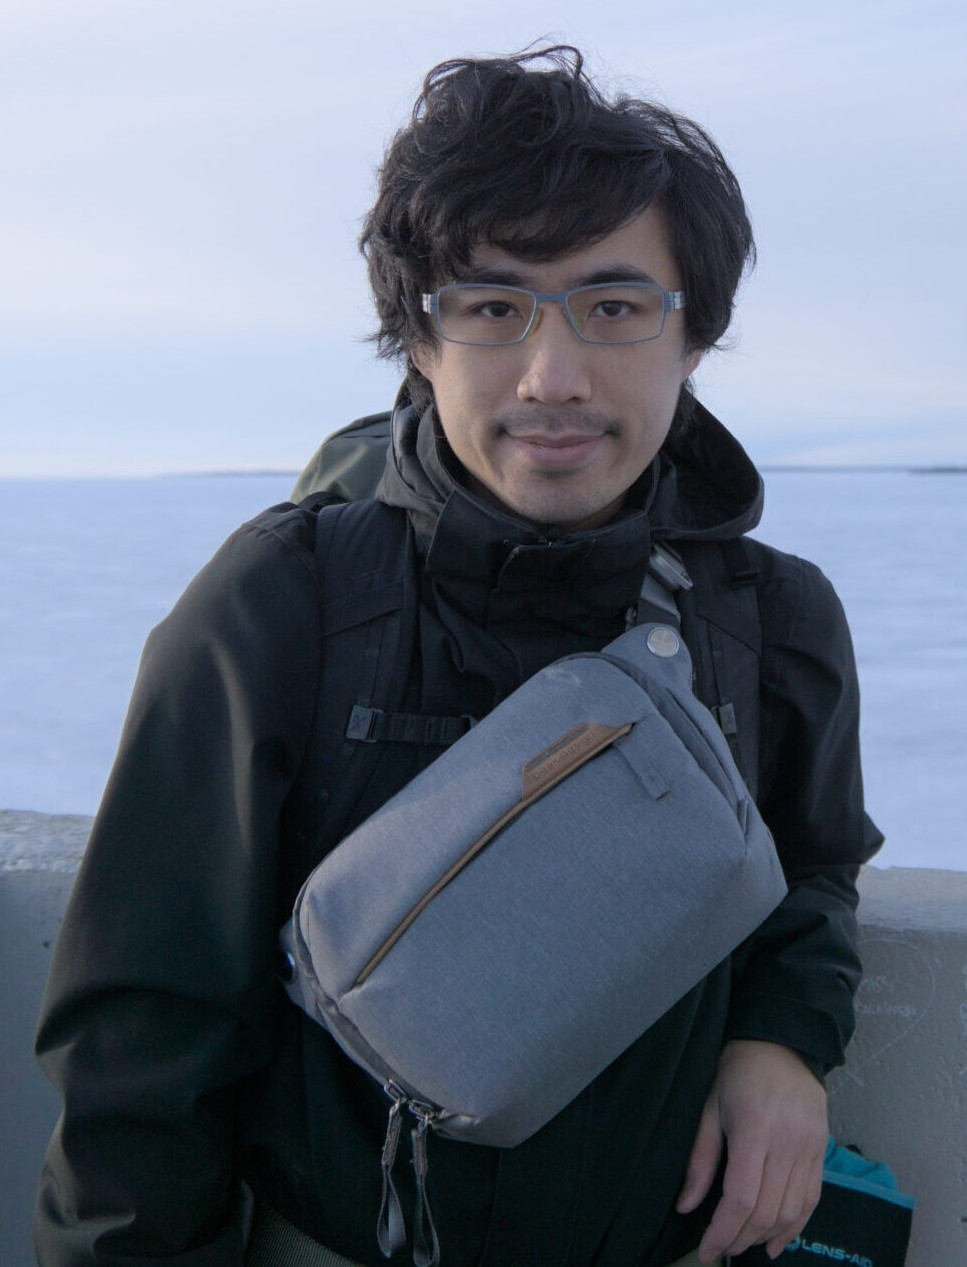
\includegraphics[keepaspectratio,frame,height=0.6\textheight]{./russell.jpg}
\end{center}
\end{column}


\begin{column}{0.5\columnwidth}
\begin{center}
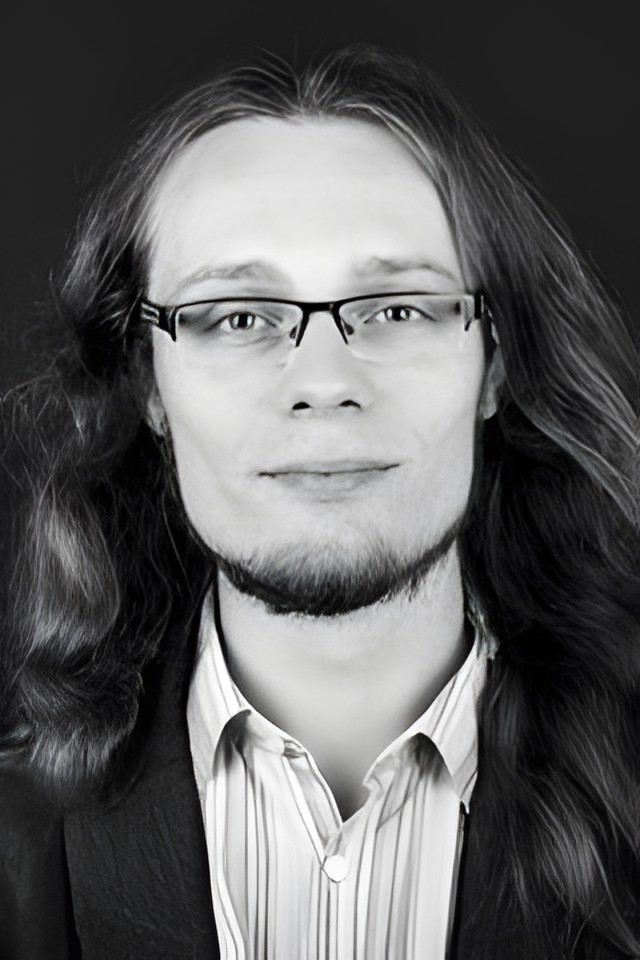
\includegraphics[keepaspectratio,frame,height=0.6\textheight]{./eamonn.jpg}
\end{center}
\end{column}
\end{columns}

\begin{center}
joint work with Russell W. F. Lai\footnote{some slides nicked from Russell.} and Eamonn W. Postlethwaite
\end{center}
\end{frame}

\begin{frame}[label={sec:orgda0b10f}]{GPV}
\begin{description}
\item[{Public Key}] Matrix \(\mat{A} \in \ZZ_q^{n \times m}\).
\item[{Secret Key}] Short basis of \(\Lambda_q^\bot(\mat{A})\) of norm \(\alpha\).
\item[{Signature of \(\mu\)}] Short vector \(\vec{u}\) satisfying
\[\begin{aligned}
  \mat{A} \cdot \vec{u} \equiv \mathsf{H}(\mu) \bmod q && \text{and} && \norm{\vec{u}} \leq \beta \leq \sqrt{m} \cdot \alpha
  \end{aligned}\]
where \(\mathsf{H}: \bin^{\star} \to \ZZ_q^n\) is hash function modelled as a Random Oracle.
\end{description}
\end{frame}

\begin{frame}[label={sec:org462cf43}]{Security Proof ≈ argument against signing the same \(\mu\) twice:}
\begin{itemize}
\item Signing same \(\mu\) twice \(\implies\)
\[\begin{aligned}
  \mat{A} \cdot \vec{u}_0 \equiv \mat{A} \cdot \vec{u}_1 &= \mathsf{H}(\mu) \bmod q, \\
  \mat{A} \cdot (\vec{u}_0 - \vec{u}_1) &= \vec{0} \bmod q,
  \end{aligned}\]
i.e. gives away short vector \(\vec{x}_0 - \vec{x}_1 \in \Lambda_q^\bot(\mat{A})\).
\item Many \(\mu\) \(\implies\) adversary gets short(-ish) basis of \(\Lambda_q^\bot(\mat{A})\) of norm \(\leq \sqrt{2\,m} \cdot \alpha\).
\end{itemize}

\begin{alertblock}{Does this (really) help adversary forge signatures?}
One-more-ISIS assumption suggest "no"!
\end{alertblock}
\end{frame}

\begin{frame}[label={sec:org6c7463d}]{The \(k\)-hint Inhomogeneous Short Integer Solution Problem:}
\begin{definition}[k-H-ISIS]
Let \(k,n,m,q,\beta,\mathsf{Dist}\), where
\[\begin{aligned}
  \forall~\mat{A} \in \ZZ_q^{n \times m},~\mathsf{Dist}(\mat{A}) \subseteq_k \Lambda_q^\bot(\mat{A}) && \text{and} && \beta^{\star} \leq r \cdot \norm{\mathsf{Dist}(\mat{A})}          
  \end{aligned}
\]
for some ratio \(r \leq \mathsf{polylog}(m)\).\footnote{We mostly care about \(r \leq O(1)\) or at least \(r \leq O(\log m)\).}

Given \((\mat{A} \sample \ZZ_q^{n \times m}, \vec{y} \sample \ZZ_q^n, \mat{U} \sample \mathsf{Dist}(\mat{A}))\) find
\(\vec{u}^{\star} \in \ZZ^m\) such that \(\mat{A} \cdot\vec{u}^{\star} \equiv \vec{y} \bmod q\) and \(\norm{\vec{u}^\star} \leq \beta^{\star}\).
\label{def:khISIS}
\end{definition}

\textbf{\(k\)-hint (Homogeneous) Short Integer Solution (k-H-SIS) Problem}: Same thing but \(\vec{y} = \vec{0}\).
\end{frame}

\begin{frame}[label={sec:org1b0f388}]{Successive Minima and SIVP}
\begin{itemize}
\item Successive minima \(\lambda_i(\Lambda) =\) radius of smallest ball containing \(i\) linearly independent lattice vectors.

\item \(\SIVP_\gamma\): Given lattice \(\Lambda \subseteq \RR^m\), find \(m\) linearly independent lattice vectors of norm at most \(\gamma \cdot \lambda_m(\Lambda)\).
\end{itemize}
\end{frame}

\begin{frame}[label={sec:org6f87155}]{Enumeration and Sieving}
Two types of lattice algorithms for \(\gamma \leq \poly[m]\):

\begin{columns}[t]
\begin{column}{0.45\columnwidth}
\begin{alertblock}{Enumeration-type}
\begin{itemize}
\item Enumerate over all non-zero vectors in \(\Lambda\) of norm at most \(\beta\).
\item Output the shortest vector.
\end{itemize}
\end{alertblock}
\end{column}

\begin{column}{0.45\columnwidth}
\begin{alertblock}{Sieving-type}
\begin{itemize}
\item Start with a long list of vectors in \(\Lambda\).
\item Search for an integer combination of vectors in the list which gives a shorter vector.
\item Add resulting vector to the list.
\item Repeat.
\end{itemize}
\end{alertblock}
\end{column}
\end{columns}
\end{frame}

\begin{frame}[label={sec:org487dfc5}]{Landscape}
Space-time complexity of \(\SIVP_\gamma\) over \(\Lambda_q^\bot(\mat{A})\) and for \(\gamma \leq \poly[m]\).

\begin{center}
\begin{tabular}{llll}
\toprule
Algorithms & Time & Memory & Assumptions\\[0pt]
\midrule
Enumeration & \(m^{\Theta(m)}\) & \(\poly[m]\) & -\\[0pt]
Sieving & \(2^{\Theta(m)}\) & \(2^{\Theta(m)}\) & -\\[0pt]
Sieving (this work) & \(2^{\Theta(m)}\) & \(\poly[m]\) & 1) sub. exp. OWF and 2) k-H-SIS is easy\\[0pt]
\bottomrule
\end{tabular}

\end{center}

We write "\((\tau,\mu)\)-algorithm" for algorithms running in time \(\tau\) and memory \(\mu\).

\begin{alertblock}{Our Interpretation}
Hinted lattice problems seem hard.
\end{alertblock}
\end{frame}

\begin{frame}[label={sec:org60d0161}]{Step 1: Entropic Reduction from k-H-SIS to k-H-ISIS}
We show that the classic SIS to ISIS reduction gives the following:

\begin{alertblock}{k-H-SIS → k-H-ISIS}
Let \(\adv\) be PPT adversary against k-H-ISIS, then there exists a PPT adversary \(\bdv\) against k-H-SIS. The output of \(\bdv\) follows a Gaussian distribution with some centre with high min-entropy.
\end{alertblock}

\(\bdv\)'s outputs are drawn from the following distribution:

\begin{itemize}
\item Sample from \(\vec{g} \gets \ddv_{\ZZ^m, s}\), where the Gaussian parameter \(s\) whp satisfies \[s \geq \sqrt{m} \cdot \lambda_m(\Lambda_q^\bot(\mat{A})) \geq \eta_{\epsilon}(\Lambda_q^\bot(\mat{A})).\]
\item Use \(\adv\) to choose a centre \(\vec{c}\) from some distribution.
\item Write and output \(\vec{g} - \mathbf{c} \sim \ddv_{\Lambda_q^\bot(\mat{A}), s, -\vec{c}}\).
\end{itemize}
\end{frame}

\begin{frame}[label={sec:org687fb4f}]{Step 2: Gaussian Vectors Generate the Lattice}
We prove the following lattice generation theorem:

\begin{alertblock}{Gaussian vectors generate the lattice}
Let \(\Lambda \subseteq \RR^m\) be any lattice and suppose \(s \geq \sqrt{m} \cdot \lambda_m(\Lambda)\).\\[0pt]
Let \(\vec{x}_i \sample \ddv_{\Lambda,s,\vec{c}_i}\) for \(i = 1,2,\ldots,t\) with arbitrary and potentially distinct centres \(\vec{c}_i\).\\[0pt]
There exists \(t^* = O(m \cdot \log(s \sqrt{m}))\) s.t. if \(t \geq t^*\), then \(\set{\vec{x}_i}_{i\in \{1 \ldots t\}}\) generates \(\Lambda\) with probability at least \(1-2^{-\Omega(m)}\).
\end{alertblock}

This was known only for \(\vec{c}_i \coloneqq \vec{0}\).\footfullcite{SODA:HavReg14}
\end{frame}

\begin{frame}[label={sec:org4188a90}]{Step 3: Improved Analysis of Sieves}
We prove the following sieving theorem:

\begin{alertblock}{Number of points in a ball}
Let \(S = \set{\vec{x}_1, \ldots, \vec{x}_t} \subseteq \RR^m\) be any set of \(t\) distinct vectors of norm \(\norm{\vec{x}_i} \leq \beta\).\\[0pt]
Let \(1 < \combinedfactor\) be some improvement ratio.\\[0pt]
There exists \(t^* \leq 2^{O(m \log \combinedfactor)}\) s.t., if \(t \geq t^*\), then there exist \(i,j\) s.t. \(0 < \norm{\vec{x}_i - \vec{x}_j} \leq \beta/\combinedfactor\).
\end{alertblock}

Previous sieve analyses were
\begin{itemize}
\item heuristic (assuming vectors are uniformly distributed on the surface of a sphere) and
\item only for \(\combinedfactor = O(1)\).
\end{itemize}
\end{frame}

\begin{frame}[label={sec:org105ca1e}]{Step 4: Finding One Mildly Short Vector}
Suppose there exists a PPT entropic k-H-SIS solver \(\bdv\) with ratio \(\growthfactor > 1\).

We construct a \((2^{O(m)},\poly[m])\) k-H-SIS solver \(\bdv'\) with constant ratio \(1/\shrinkfactor < 1\).

\begin{alertblock}{Basic Idea}
Run entropic kHSIS solver \(\bdv\) many times to get \(2^{\Omega(m)}\) vectors, then apply sieving theorem.
\end{alertblock}
\end{frame}

\begin{frame}[label={sec:orgfc84649}]{Step 4: Finding One Mildly Short Vector (More Details)}
\begin{enumerate}
\item Success probability amplification: Repeat \(\bdv\) to make success probability overwhelming.
\item Randomised memory-inefficient sieve:
\begin{itemize}
\item Fill random tape of (amplified) \(\bdv\) with \(t \geq 2^{\Omega(m)}\) independent randomness \(\rho_1, \ldots, \rho_t\).
\item For each \(i,j \in [t]\):
\begin{itemize}
\item Compute \(\vec{x}_i \gets \bdv(\mat{A}, \mat{U}; \rho_i)\).
\item Compute \(\vec{x}_j \gets \bdv(\mat{A}, \mat{U}; \rho_j)\).
\item Output \(\vec{x}_i - \vec{x}_j\) if \(0 < \norm{\vec{x}_i - \vec{x}_j} \leq 1/\shrinkfactor \cdot \norm{\mat{U}}.\)
\item Entropic-ness of \(\bdv\) + sieving theorem \(\implies\) Successful output with overwhelming probability.
\end{itemize}
\end{itemize}
\item Derandomisation: derandomise the double-loop with sub-exp. secure PRF.
\end{enumerate}
\end{frame}

\begin{frame}[label={sec:orge20e686}]{Step 5: Finding Lots of Mildly Short Vectors}
Suppose further that the entropic kHSIS solver \(\bdv\) has Gaussian outputs.

We construct a \((2^{O(m)}, \poly[m])\) sieving routine \(\cdv\):

\begin{description}
\item[{Input}] \((\mat{A}, \mat{U})\) where \(\mat{U}\) generates \(\Lambda_q^\bot(\mat{A})\).
\item[{Output}] \(\mat{U}' \subset \Lambda_q^\bot(\mat{A})\) generating \(\Lambda_q^\bot(\mat{A})\) with \(\norm{\mat{U}'} \leq 1/\shrinkfactor \cdot \norm{\mat{U}}\).
\end{description}

\begin{block}{Basic Idea}
Run \(\bdv'\) many times to get \(\Omega(m \cdot \log(s \sqrt{m}))\) vectors, then apply lattice generation theorem.
\end{block}

\begin{itemize}
\item Need to be able to argue about output distribution.
\end{itemize}

\begin{alertblock}{Key Idea}
Do not sieve over \(\vec{g}_{i} - \vec{c}_{i}\) but over \(\vec{c}_{i}\) in \((\vec{g}_{i}, \vec{c}_{i})\)
\end{alertblock}
\end{frame}

\begin{frame}[label={sec:org1c14394}]{Step 6: Iterated Sieving}
\textbf{Assume} the existence of a chain of entropic k-H-SIS solvers \(\bdv_1, \bdv_2, \ldots\) with Gaussian outputs with arbitrary (small) centres, accepting Gaussian inputs with arbitrary (small) centres.

We construct a \((2^{O(m)}, \poly[m])\) algorithm solving \(\SIVP_\gamma\) for \(\Lambda_q^\bot(\mat{A})\) with \(\gamma \geq m\).

\begin{block}{Basic Idea}
Feed output of sieving subroutine to itself until improvement stops.
\end{block}

\begin{itemize}
\item Assume each \(\bdv_{i}\) succeeds with probability \(2^{-O(m/\mathsf{polylog}(m))}\)
\item Run chain of length \(\log(m)\) to reduce norm by factor \(2 \cdot \sqrt{m} \cdot \omega(\log(m))\)
\item Use discrete Gaussian sampler to produce "fresh" clean hints by factor \(\sqrt{m} \cdot \omega(\log(m))\) larger
\item "Zig-zag" down
\end{itemize}
\end{frame}

\begin{frame}[label={sec:org202f007}]{I lied!}
\begin{center}

\includegraphics[keepaspectratio,height=.9\textheight]{./sis-with-hints-real.jpg}
\end{center}
\end{frame}

\begin{frame}[label={sec:orgc779573},standout]{Fin}
\begin{center}
\huge

\begin{description}
\item[{Designers}] Please consider whether you can re-use one of those many newfangled assumptions before introducing yet another one.

\item[{Cryptanalysts}] Analyse them!
\end{description}
\end{center}
\end{frame}
\end{document}
